\documentclass[letterpaper, 10 pt, conference]{ieeeconf}

\usepackage[utf8]{inputenc}
\usepackage{acronym}
\usepackage[natbib=true,backend=bibtex,firstinits=true,style=numeric-comp,defernumbers,maxnames=99,maxcitenames=2]{biblatex}
\usepackage{amsmath}
\usepackage{mathptmx} % amsmath makes the paper longer
\usepackage{pgfplots}
%\usepackage{subfig}

\bibliography{cdc}

\IEEEoverridecommandlockouts
\overrideIEEEmargins

% options for pgfplots
\pgfplotsset{compat=1.8,compat/show suggested version=false}
\usetikzlibrary{plotmarks}
\usetikzlibrary{calc}
% begin of externalization
\usetikzlibrary{external}
%\tikzexternalize

\newcommand{\str}[1]{{\color{blue} \scriptsize \sf\selectfont @#1@}}

% acronym definitions
\acrodef{lc}[LC]{Local Controller}
\acrodefindefinite{lc}{an}{a}
\acrodef{vm}[VM]{Virtual Machine}
\acrodef{rm}[RM]{Resource Manager}
\acrodefindefinite{rm}{an}{a}
\acrodef{ip}[IP]{Infrastructure Provider}
\acrodef{sp}[SP]{Service Provider}
\acrodefindefinite{sp}{an}{a}

% =============================================================================
\title{\LARGE \bf Load-balancing Adaptive Cloud Applications}
\author{Authors} 
% =============================================================================


\begin{document}

\maketitle
\thispagestyle{empty}
\pagestyle{empty}

\begin{abstract}

\end{abstract}

\section{Introduction}
\label{sec:introduction}
Cloud computing is expected to be one of the driving force of the
future economy~\citep{WPonMckinsey13}. Already, it has dramatically
changed the management of computing infrastructures. On one hand,
public infrastructure providers, such as Amazon EC2, allow service providers to deploy
their services on large infrastructures with no up-front
cost~\citep{Buyya09:FGCS}. On the other hand, the flexibility offered
by cloud technologies themselves favors the adoption of private
clouds~\citep{Gulati11:HotCloud}, therefore, self-hosting service providers themselves are converting
their computing infrastructures into small, internally-managed
clouds.

One of the main advantages offered by cloud infrastructures is {\bf
  elasticity}. A service provider that wants to deploy a new service on the
cloud can rapidly provision the required computing resources,
automatically acquiring and releasing computing resources as
required~\citep{Herbst13:ICAC}.  Elasticity can be of two
complementary types: vertical and horizontal. Vertical elasticity
consists in adding or removing resources (e.g., CPU cores) from an
existing \ac{vm}, while horizontal elasticity deals with changing the
number of \acp{vm} allocated to a specific service, adding a new
machine or removing an existing one.
%
Horizontal elasticity calls for the introduction of a specialized
component, called {\bf load-balancer}, that takes care of routing the
end-user requests to one of the \acp{vm} composing the service. Load-balancing
techniques have been widely studied and
adopted~\citep{Barroso09,Lu11:PerfEval,Lin12:IGCC,BeesBased:ADAPTIVE}.

One of the main issues with cloud computing infrastructures, however,
is {\bf robustness} to unexpected events. For example, flash-crowds
are sudden increases of end-users, that may increase the required
capacity by up to five times~\citep{Bodik10:SoCC}. Similarly, hardware
failures may temporarily reduce the capacity of the infrastructure, while
the failure is repaired~\citep{Barroso09}. Due to the large magnitude
and short duration of such events, it may be economically too costly
to keep enough spare capacity to properly deal with them. As a result,
unexpected events may lead to infrastructure overload, which translates
to unresponsive services, leading to dissatisfied end-users
and revenue loss.

Cloud services therefore greatly benefit from
self-adaptation techniques~\cite{SalehieSelfadaptive:TAAS}, such as
{\bf brownout}~\citep{cloudish-tr}. A brownout service
adapts itself by reducing the amount of computations it executes
to produce a response, so as to maintain response time around a given setpoint.
In essence, some computations are
marked as mandatory --- for example, the display of the product
information in an e-commerce website --- while others are optional ---
for example, the display of recommendations of similar products.
Whenever an end-user request is received, the service can choose to execute
or not the optional code based on the capacity available to it,
to which it adapts by monitoring response times. Note that executing optional code directly
translates into a better service for the end-user and more revenues for
the service provider. This approach proved to be successful for dealing with
unexpected events. However, brownout services were composed
of a single replica, running inside a single \ac{vm}.

In this paper, we extend the brownout paradigm to services featuring
multiple replica, hosted inside individual \acp{vm}. We develop
a load-balancer that takes into account the replica
adaptation to decide how to forward requests to replicas.
Besides enabling horizontal elasticity, having a load-balancer and multiple replicas
makes services fault-tolerant. Existing, state-of-the-art
load-balancers may forward requests based on the response-time of each
replica, which leads to inefficient decisions for brownout services.
Indeed, such services already keep their response-time
at a given setpoint, at the expense of reducing the amount of optional
content served. Hence, by measuring response-time alone, it is not possible
to discriminate between a replica that is avoiding overload by not
executing the optional code and a replica that is not threatened with
overload executing all optional code, both achieving low response
times.  Therefore, existing load-balancing techniques that monitor
response times should be improved to migrate load away from replicas
not executing optional code.

Our challenge is to find a load-balancing methodology that maximizes
the amount of served optional content, provided that every replica
independently serves only an amount of optional content that allows it
to maintain the maximum response time below a configured target.

Our contribution is summarized as follows.
\begin{itemize}
\item We discuss load-balancing architectures and the required
  enhancements to the replicas that allow to deal with
  brownout services efficiently.
\item We propose two load-balancing policies that aim at maximizing
  the performance of brownout services, in terms
  of frequency of execution of the optional code, therefore
  maximizing the total revenue for the service provider.
\item We evaluate existing load-balancing strategies and compare them
  with the two proposed approaches, demonstrating the need for a
  brownout-aware load-balancer and showing that the proposed policies
  outperform existing techniques.
\end{itemize}


\section{Related Work}
\label{sec:related}
\textcolor{blue}{\textit{\textbf{Martina:} All the following is just a
    bunch of comments that I have put together. (1): it is not written
    in decent English but I hope it is understandable anyway. It is
    not intended to be quality writing but just represent a bunch of
    notes that we should take into account when generating the related
    work. (2) So far I have scratched basically only the old
    literature, so don't consider it exhaustive by any means.}}

Load balancing has been explored exensively and different strategies
have different aims. For example, electricity based load balancing
proposes to reduce the amount of consumed electricity by directing the
requests to different replicas based on the electricity price
market~\cite{LoadBalancingForElectricity:TCC}.

In the software engineering context load balancing is often called
dynamic binding, so check the literature for that too.

In general it can be divided into different types. Static load
balancing refers to a fixed policy on a fixed system. Not only the
number of replicas is always the same but also the policy used to
select where to direct the traffic is always the same. This found many
applications early on, for example in load sharing on multiprocessor
systems~\cite{StaticLoadBalancing:TSE,StaticOptimal:ACM}.

We are not interested in static load balancing, because we want to
account for variability, both in the number of replicas and in their
behavior. Our replicas, in fact can join the system later on ---
therefore taking into account autoscaling mechanism that are nowadays
popular in cloud computing --- and can be self-adaptive in nature, in
the sense that they can adjust their behavior to match specific
quality of service requirement like maximum or average latency
ones. 

In dynamic load balancing we distinguish two categories. One where the
number of replicas and their behavior is assumed to vary over time but
the policy is static --- for example the Round Robin load balancing
where the requests are distributed irregardless of the load on the
involved replicas and of their status. See if we have examples for
this one beside the simple Round Robin case, in case cite them
here. Also this category is not related to our work, since we assume
that we want to exploit the variations that are happening at the
replica level. However, it would be nice to have implemented a couple
of these policies (if we can find some of them) to demonstrate that we
need to account for the variability.

The second category is when the load balancing policy takes into
account variations happening at the replica level --- for example,
when it takes into account the replica response times to decide where
to send the next request. Many approaches fall in this category. For
example, in old times, Stankovic proposed a Bayesian
approach~\cite{Stankovic:TC} to solve this problem. In his solution,
an estimator of the queue lenght per replica (in his case per
processor because cloud computing was not invened yet) is kept updated
and the next job is sent to the least congested replica. This
algorithm is very unlikely to work in our case because it has no
knowledge of the adaptation that the single replica is preforming, but
we borrow from the idea of having the replicas communicating some
indicator of their behavior, and use it to communicate the dimmer
value. It would be nice to have this as a comparison point, although
it is from the 80s, we can simply feedback the number of elements in
the queue and see if that helps --- maybe we would get similar
results, although not by construction.


\section{Problem Statement}
\label{sec:problem}
Load-balancing problems can be formulated in many ways. This is
especially true for the case addressed in this paper where the
load-balancer should distribute the load to adaptive entities, that
play a role by themselves in adjusting to the current situation. This
section discusses the characteristics of the considered infrastructure
and clearly formulate the problem under analysis.

\begin{figure}[t]
  \centering 
  \usetikzlibrary{arrows}
\usetikzlibrary{automata}
\usetikzlibrary{positioning}
\usetikzlibrary{backgrounds}
\usetikzlibrary{fit}

\tikzset{
    state/.style={
           rectangle,
           rounded corners,
           draw=black, very thick,
           minimum height=0.6cm,
           minimum width=1.3cm,
           inner sep=3pt,
           text centered,
           node distance=1.8cm,
           },
    process/.style={
           rectangle,
           rounded corners,
           draw=black, very thick,
           minimum height=0.6cm,
           minimum width=1.3cm,
           inner sep=3pt,
           text centered,
           %node distance=1cm,
           },
    newprocess/.style={
           rectangle,
           rounded corners,
           draw=black, very thick,
           fill=lightgray,
           minimum height=0.6cm,
           minimum width=1.3cm,
           inner sep=3pt,
           text centered,
           %node distance=1cm,
           },
    processplaceholder/.style={
           minimum height=0.6cm,
           minimum width=1.3cm,
           %inner sep=3pt,
           text centered,
           %node distance=1cm,
           },
    closerstate/.style={
           rectangle,
           rounded corners,
           draw=black, very thick,
           minimum height=0.5cm,
           minimum width=5.35cm,
           inner sep=3pt,
           text centered,
           node distance=1.1cm,
           },
    abovish/.style={
           rectangle,
           rounded corners,
           draw=none,
           minimum width=1.3cm,
           text centered,
           node distance=1.3cm,
           },
    supercloserstate/.style={
           rectangle,
           draw=none,
           minimum height=0.2cm,
           minimum width=6.9cm,
           node distance=1cm,
           },
}

\begin{tikzpicture}[font=\small]
\tikzstyle{surround} = [fill=black!20,very thick,draw=black,rounded corners, inner sep=5pt,]
\tikzstyle{surroundblue} = [fill=blue!20,very thick,draw=black,rounded corners, inner sep=5pt,]
\tikzstyle{surroundyellow} = [fill=yellow!20,very thick,draw=black,rounded corners, inner sep=5pt,]
\tikzstyle{external} = [fill=none,very thick,draw=black,rounded corners, inner sep=15pt,]

% clients
\node[process] (clients){clients};

% load-balancer
\node[newprocess, right=1cm of clients] (lb){load-balancer};

% servers
\node[processplaceholder, right=1cm of lb] (replicaI) {$\vdots$};
\node[process, above=0cm of replicaI] (replica1) {$\text{replica}_1$};
\node[process, below=0cm of replicaI] (replicaN) {$\text{replica}_n$};

% controllers
\node[processplaceholder, right=1cm of replicaI] (controllerI) {$\vdots$};
\node[process, right=1cm of replica1] (controller1) {$\text{controller}_1$};
\node[process, right=1cm of replicaN] (controllerN) {$\text{controller}_n$};

% clients to lb
\draw[thick,->] (clients.east) -- (lb.west) node[midway, above] {$\lambda$};

% lb to replicas
\draw[thick,->] (lb.east) -- (replica1.west) node[midway, above] {$\lambda_1$};
\draw[thick,->] (lb.east) -- (replicaN.west) node[midway, above] {$\lambda_n$};

% replica to controllers
\draw[thick,->] ([yshift=+1mm]replica1.east) -- ([yshift=+1mm]controller1.west) node[midway, above] {$t_1$};
\draw[thick,<-] ([yshift=-1mm]replica1.east) -- ([yshift=-1mm]controller1.west) node[midway, below] {$\theta_1$};
\draw[thick,->] ([yshift=+1mm]replicaN.east) -- ([yshift=+1mm]controllerN.west) node[midway, above] {$t_n$};
\draw[thick,<-] ([yshift=-1mm]replicaN.east) -- ([yshift=-1mm]controllerN.west) node[midway, below] {$\theta_n$};

\end{tikzpicture}
 
  \caption{Architecture of a brownout-compliant cloud application
    featuring multiple replicas.}
  \label{fig:architecture}
\end{figure}

Figure~\ref{fig:architecture} illustrates the software architecture
that is deployed to execute a brownout-compliant application composed
by multiple replicas. Despite the modifications needed to make it
brownout-compliant, the architecture is widely accepted as the
reference one for cloud applications~\citep{Barroso09}.

In a generic load-balancing infrastructure, clients generate traffic
to the cloud application at an unpredictable but measurable rate
$\lambda$. The traffic is directed to a load-balancer that sorts it,
sending requests to the different $n$ replicas. Each replica $i$
receives a fraction $\lambda_i$ of the incoming traffic and implements
the application logic. Clearly, since the load balancer is redirecting
the entire pool of received requests, $\sum_i \lambda_i = \lambda$.
It is also possible to formulate the problems using replica weights.
In this case, each replica receives requests at a rate $\lambda_i =
w_i \cdot \lambda$, such that $\sum_{i} w_i = 1$. In this case, the
load balancer simply computes the \textbf{replica weights} $w_i$
according to its load-balancing policy.

Special to our case is the presence of a controller within each
replica~\cite{cloudish-tr}. This controller takes care of adjusting
the percentage of requests served with the optional components enabled
based on the measured response time of the requests served by the
replica. The controller for replica $i$ receives a vector of response
times $t_i$ (the average value can be used, as well as the maximum one
or the 99th percentile, depending on what the requirements on the
control systems are) and produces the percentage $\theta_i$ of
requests that should be served with optional components in the next
time interval.

In fact, a replica $i$ responds to requests either partially, where
only mandatory content is included in the reply, or fully, where both
mandatory and optional content is included. The service rate for a
partial response is $\mu_i$ while a full response is generated with a
rate $M_i$. Obviously, partial replies are faster to compute than full
ones, since the optional content does not need to be prepared, hence,
$\mu_i \geq M_i$. Assuming the replica is not saturated, it serves
requests fully at a rate $\lambda_i \cdot \theta_i$ and partially at a
rate $\lambda_i \cdot (1-\theta_i)$. An existing load-balancer based
on response times analysis would hardly work with brownout-compliant
applications, due to their self-adaptivity and the selection of the
value $\theta_i$.

Many alternatives can be envisioned on how to extend existing load
balancers to deal with brownout-compliant applications.

In the first case, the load-balancer does not know anything about the
current state of the system but can inspect the requests and the
responses and see how many of them have been executed with the
optional components turned on. This would give it an estimation of the
probability of executing optional code $\theta_i$ per replica but not
the certainty of its current value, due to the probabilistic setup.

In the second case, the load-balancer does not know anything about the
state of the system and cannot inspect the requests because this would
be too heavy on the architecture, therefore it can try to estimate the
probability of executing optional code based on the time needed to
compute the response --- clearly, a request with optional code enabled
would take longer than one without it. The estimate of $\theta_i$ in
this case would be less accurate than in the previous scenario.

In the third scenario, the load-balancer receives information about
$\theta_i$ from the replicas. This solution is lighter than the others
on the load balancer side but requires additional communication. The
overhead, however, is very limited, since only one value should be
reported per replica. For the purposes of this paper, we assume that
to aid load-balancing decisions, each replica piggy-backs the current
value of $\theta_i$ through the reply, so that this value can be
observed by the load-balancer, limiting the overhead. The parameters
$\theta_i$ are computed by controllers based on a target average or
maximum response time $\bar{\tau}$. Each replica $i$ periodically
reports the average observed vector of response-times $t_i$ to its
controller. In exchange, the controller adjusts $\theta_i$ to maintain
the desired response-time close to its target value. The load-balancer
does not have any knowledge on \emph{how} each replica controller
adjusts the percentage $\theta$, it can only know its reported value.

Within this architecture, we want to solve the problem of designing a
{\bf load-balancer policy}. Knowing the values of $t_i$ and $\theta_i$
for each replica $i \in [1, n]$ and the current (assumed constant)
arrival rate $\lambda$, a load-balancer should compute the values of
the weights $w_i$ such that
\begin{equation}
\sum_{i} \lambda w_i \theta_i = \lambda \sum_i w_i \theta_i
\end{equation}
is maximized. In other words, the load-balancer should maximize the
amount of requests served with the optional part enabled. In practice,
this would also maximize the application owner's revenue.


\section{Solution}
\label{sec:solution}
This section describes three different solutions for balancing the
load directed to self-adaptive brownout-compliant applications
composed of multiple replicas. The first two strategies are heuristic
solutions that take into account the self-adaptivity of the
replicas. The third alternative is based on optimization theory, with
the aim of providing guarantees on the best possible behavior. In all
solutions, the load-balancer is configured with a control period of
$1$s.

\subsection{Variational principle-based heuristic (VPBH)}

Our first solution is inspired by the predictive approach described,
in Section~\ref{sec:related}. The core of the predictive solution is
to examine the variation of the involved quantities. While in its
classical form, this solution relies on variations of response times
or pending request count per replica, our solution is based on the how
the control variables $\theta_i$ are changing.

If the percentage $\theta_i$ of optional content served is increasing,
the replica is assumed to be less loaded, and more traffic can be sent
to it. On the contrary, when the optional content decreases, the
replica will receive less traffic, to decrease its load and allow it
to increase $\theta_i$.

The replica weights $w_i$ are initialized to $\frac{1}{n}$ where $n$
is the number of replicas. The load-balancer periodically updates the
values of the weights based on the values of $\theta_i$ received by
the replicas. At time $k$, denoting with $\Delta \theta_i (k)$ the
variation $\theta_i (k) - \theta_i (k-1)$, the solution computes a
potential weight $\tilde{w}_i(k+1)$ according to
\begin{equation}
  \tilde{w}_i(k+1) = w_i(k) \cdot 
\left[ 1 + \gamma_p \, \Delta \theta_i (k) + \gamma_i \, \theta_i (k) \right] ,
\label{eq:theta-diff}
\end{equation}
where $\gamma_p$ and $\gamma_i$ are constant gains, respectively
related to a proportional and an integral load-balancing action. As
calculated, $\tilde{w}_i$ values can be negative. This is clearly not
feasible, therefore negative values are truncated to a small but still
positive weight. Using a positive weight instead of zero allows us to
probe the replica and see whether it is favorably responding to new
incoming requests or not. Moreover, the computed values do not respect
the constraint that their sum is equal to 1, so they are then
re-scaled according to
\begin{equation}
  w_i (k) = \cfrac{\tilde{w}_i (k)}{\sum_i \tilde{w}_i (k)}.
\label{eq:theta-diff-rescale}
\end{equation}

We selected $\gamma_p = 0.5$ based on experimental results. Once
$\gamma_p$ is fixed to a selected value, increasing the integral gain
$\gamma_i$ calls for a stronger action on the load-balancing side,
which means that the load-balancer would take decisions very much
influenced by the current values of $\theta_i$, therefore greatly
improving performance at the cost of a more nervous control action. On
the contrary, decreasing $\gamma_i$ would stabilize the control
signal, possibly resulting in performance loss due to a slower
reaction time. The choice of the integral gain allows to exploit the
trade-off between performance and robustness. For the experiments we
chose $\gamma_i = 5.0$.

\subsection{Equality principle-based heuristic (EPBH)}

The second policy is based on the following heuristic: In the best
conditions, every replica should have a similar behavior. Based on his
heuristic, the control variables $\theta_i$ should be as close as
possible to one another. In fact, if the values of $\theta_i$ converge
to a single value, this means that the traffic is routed so that each
replica can serve the same percentage of optional content, i.e., the
most powerful replica is receiving more traffic with respect to the
least powerful one. The distribution should ideally allow to converge
to a value that is maximum with the entire pool of requests received
by the application. This approach therefore selects weights that would
encourage the control variables $\theta_i$ to converge to a single
value.

The policy computes a potential weight $\tilde{w}_i(k+1)$
\begin{equation}
  \tilde{w}_i(k+1) = w_i(k) + \gamma_e e_i(k)
\label{eq:equal-thetas}
\end{equation}
where
$$e_i(k)=\left[ \theta_i (k) - \cfrac{\sum_j \theta_j (k) }{n} \right]$$
and $\gamma_e$ is a non-zero positive parameter of the algorithm which
accounts for how fast the algorithm should converge. For the
experiments we chose $\gamma_e = 0.025$. The weights are simply
modified proportionally to the difference between the current control
value and the average control value set by the replicas. Clearly, the
same saturation and normalization described in Equation
\eqref{eq:theta-diff-rescale} have to be applied to the proposed
solution, to ensure that the sum of the weights is equal to one and
that they have positive values --- i.e., that all the incoming traffic
is directed to the replicas and that each replica receives at least
some requests.

By inserting the expression for $\tilde w_i$ from
\eqref{eq:equal-thetas} in the normalization equation
\eqref{eq:theta-diff-rescale} we get
\begin{equation}
  w_i(k+1)=\cfrac{w_i(k)+\gamma_ee_i(k)}{\sum_jw_j(k)+\gamma_e\sum_je_j(k)} .
\label{eq:weights}
\end{equation}

% Since we normalized all weights $w_i(k)$ to sum to one
% ($\sum_jw_j(k)=1$), and
% $$\sum_je_j(k)=\sum_j\left[\theta_j(k)-\frac{\sum_l\theta_l(k)}{n}\right]=0$$
% we get that \eqref{eq:weights} in stationarity is
% $$w_i(k)=w_i(k)+\gamma_ee_i(k)$$
% and the only solution for this is that $e_i(k)=0$, all dimmers are
% equal in stationarity.

\subsection{Optimization based load-balancing (OBLB)}

The third approach is to update the replica weights based on the
solution of an optimization problem, where the objective is to
maximize the quantity denoted by Equation~\eqref{eq:objective}.

In this solution, each replica is modeled as an $M/G/1$ queue with a
Processor Sharing (PS) discipline. The arrival clients are Markovian
(M) processes, the service times have a general (G) distribution and
each replica consists of a single server. According to the processor
sharing discipline, all clients are served immediately after their
arrival and share a fraction of the available computation power.

\str{Explain why M/G/1 and not M/G/n where n would be the number of
  cores available for the replica. Kind of due to the PS discipline,
  but need better explaination. Also, Karl-Erik commented that we
  cannot assume that control people know what an M/G/1 queue
  is. Background should be better explained.}

We use a general distribution for service times to account for the
brownout adaptation. For each replica $i$ we define $f_{S_i}$, the
probability density function for service times $S_i$, as
\begin{align}
  f_{S_i} (t) = (1 - \theta_i) \cdot \mu_i \cdot e^{-\mu_i \cdot t} +
  \theta_i \cdot M_i \cdot e^{-M_i \cdot t} ,
\label{eq:pdf-servicetimes}
\end{align}
where $t$ represents time, $\theta_i$ is the probability of activating
the optional components, $\mu_i$ denotes the service rate for requests
that do not have optional components enabled and $M_i$ is the service
rates for requests where the optional part is computed. Therefore, the
expression~\eqref{eq:pdf-servicetimes} is a mixture of two
exponentially distributed service times corresponding to serving all
clients with or without optional content. It is well known that for $M/G/1$ queues adopting the processor sharing discipline, the mean response times will only depend on the mean of the service time distribution~\cite{kleinrock67},~\cite{sakata71}, with an effective service rate for each replica $i$ given by
\begin{equation}
  \mu_i^* = \left[ E[S_i] \right]^{-1} = \left[ \frac{1-\theta_i}{\mu_i}
    + \frac{\theta_i}{M_i} \right]^{-1} .
  \label{eq:effective-service-rate}
\end{equation}

It is possible to compute the value of the service rate that respects
the replica objective that the mean response times $t_i$ is equal to
the desired value $t_i^*$, that is given to the brownout-compliant
replica.
\begin{equation}
  t_i = \frac{1}{\mu_i^*-\lambda w_i} = t_i^*
  \Longrightarrow \mu_i^* = \frac{1+t_i^*\lambda w_i}{t_i^*} 
  \label{eq:desired-service-rate}
\end{equation}
Combining Equation~\eqref{eq:effective-service-rate} and
\eqref{eq:desired-service-rate}, one can calculate the optimal values
$\theta_i^*$ of $\theta_i$ that would respect the response time
constraints.  Notice that these values are not used in the replicas
and are simply computed by the optimization based load-balancer as the
optimal stationary conditions for the control variables
$\theta_i$. Clearly, one could also think of using these values within
the replicas but in this investigation we want to completely separate
the load-balancing policy and the replicas internal control loops and
treat the internal loop as a fast system, converging to its stationary
conditions before the next load-balancing intervention.

The values $\theta_i^*$ are
\begin{equation}
  \theta_i^* = \frac{M_i \cdot \left( \mu_i t_i^* - 1 -\lambda w_i
      t_i^* \right)}{{\left( 1+\lambda w_i t_i^* \right) \cdot
      \left(\mu_i-M_i \right)}} = \frac{A_i - B_i w_i}{C_i + D_i w_i}.
  \label{eq:optimal-thetas}
\end{equation}
Recalling that $\theta_i$ is the probability of executing the optional
components when producing the response, the values $\theta_i^*$ should
be constrained to belong to the interval $[0, 1]$. Imposing this
condition provides the following inequalities.
\begin{equation}
  \frac{C_i-A_i}{B_i+D_i} \leq w_i \leq \frac{A_i}{B_i}
  \label{eq:constraints-optimal-thetas}
\end{equation}
Using these inequalities as constraints, it is possible to formally
state the optimization problem as
\begin{equation}
\begin{array}{rl}
  \max_{w_i} \;\;\; & J = \sum_i w_i \theta_i = \sum_i w_i  \frac{A_i - B_i w_i}{C_i + D_i w_i} \\
  \textnormal{s.t.} \;\;\; & \sum_i w_i = 1 \\
  & \max (0,\frac{C_i-A_i}{B_i+D_i}) \leq w_i \leq \frac{A_i}{B_i}
\end{array}
  \label{eq:optimization-problem}
\end{equation}

The objective function $J$ can be shown to be concave in $w_i$ and the
constraints are linear. Therefore the optimization problem is itself
concave and can be solved with standard methods \str{Citation
  needed}. We use CVXOPT, a Python solver for convex optimization, to
obtain the values of the weights.

Notice that solving the optimization
problem~\eqref{eq:optimization-problem} guarantees that the best
possible solution is found, but requires a lot of knowledge about the
single replicas. In fact, while other solutions require knowledge only
about the incoming traffic and the control variables for each replica,
the optimization-based solution relies on knowledge of the service
time of requests with and without optional content $M_i$ and $\mu_i$
that might not be available and could require additional computations
to be estimated correctly.

\str{Find out how the optimizer scales when the number of replicas
  increases and comment on that.}


\section{Evaluation}
\label{sec:evaluation}
In this section we describe our experimental evaluation, discussing
the performance indicators used to compare different strategies, the
simulator developed and used to emulate the behavior of
brownout-compliant replicas driven by the load-balancer and our case
studies.

\subsection{Performance indicators}

Performance measures are necessary to objectively compare different
algorithms. While our first performance indicator is clearly defined
as the \textbf{percentage $\%_{oc}$} of the total requests served with
the optional content enabled, we also would like to introduce some
other performance metrics to compare the implemented load-balancing
techniques.

For this, we use the \textbf{user-perceived stability
  $\sigma_u$}~\cite{GeograficalSASO}. This metric refers to the
variation of performance as observed by the users, and it is measured
as the standard deviation of response times. Its purpose is to measure
the ability of the replicas to respond timely to the client
requests. The entire brownout framework aims at stabilizing the
response times, therefore it should achieve better user-perceived
stability, regardless of the presence of the load-balancer. However,
the load-balancing algorithm clearly influences the perceived
response times, therefore it is logical to check whether the newly
developed algorithms achieve a better perceived stability with respect
to the classical ones. Together with the value of the user-perceived
stability, we also report the \textbf{average response time $\mu_u$}
to distinguish between algorithms that achieve a low response time
with possibly high fluctuations from solutions that achieve a higher
but more stable response time.

\subsection{Simulator}

To test our load-balancing strategies, together with existing state of
the art solutions, we implemented a Python-based simulator for
brownout-compliant applications. In the simulator, it is easy to
plug-in new load-balancing algorithms. The simulator is based on the
concepts of \emph{Client}, \emph{Request}, \emph{LoadBalancer},
\emph{Replica} and \emph{Link}.

When a new client is defined, it can behave according to the open-loop
client model, where it simply issues a certain number of unrelated
requests (as it is true for clients that respect the Markovian
assumption), or according to the closed-loop
one~\cite{openvsclosed}. Closed-loop clients issue a request and wait
for the response, when they receive the response they think for some
time and subsequently continue sending another request to the
application. While this second model is more realistic, the first one
is still useful to simulate the behavior of a large number of
clients. The simulator implements both models, to allow for complete
tests.

Requests are received by the load-balancer, that directs them towards
different replicas. The load-balancer can work on a per-request basis
or based on weights. The first case is used to simulate policies like
Round Robin, Random, Shortest Queue First and so on, that do not rely
on the concept of weights. The weighted load-balancer is used to
simulate the strategies proposed in this paper, as well as state of
the art solutions like the Weighted Round Robin.

Each replica simulates the computation necessary to serve the request
and chooses if it should be executed with or without the optional
components activated. If the optional content is served the service
time is a random number from a gaussian distribution with mean
$\phi_i$ and variance $0.01$, while if the optional content is not
served, the mean is $\psi_i$ and the variance is $0.001$. The
parameters $\phi_i$ and $\psi_i$ are specified when replicas are
created and can be changed during the execution. The service rate of
requests with the optional component $M_i = 1/\phi_i$ while for
serving only the mandatory part of the request the service rate is
$\mu_i = 1/\psi_i$. The replicas are also executing an internal
control loop to select their control variables, i.e., the probability
of executing the optional components. Details on the interal control
loops can be found in~\cite{cloudish-tr}. The replicas use Processor
Sharing to process the requests in the queue, meaning that each of the
$n$ active request will get $\frac{1}{n}$-th of the processing
capability of the replica.

Finally, there are network links connecting the load-balancer and the
replicas. These link are part of the simulator, to study the effect of
network delays in communicating the necessary feedback information for
the load-balancer execution.

The simulator receives as input a \emph{Scenario}, which describes
what can happen during the simulation. The scenario definition
supports the insertion of new clients and the removal of existing
ones. It also allows to turn on and off replicas at specific times
during the execution and to change the service times for every
replica, both for the optional components and for the mandatory
ones. This simulates a change in the amount of resources given to the
machine hosting the replica and it is based on the assumption that
these changes are unpredictable and can happen at the architecture
level, for example due to the cloud provider co-locating more
applications onto the same physical hardware, therefore reducing their
computation capability~\cite{Tomas13:CAC}.

With the scenarios, it is easy to simulate different working
conditions and to have a complete overview of the changes that might
happen during the load-balancing and replica execution. In the
following, we describe two experiments conducted to compare the
load-balancing strategies when subject to different execution
conditions.

\subsection{Reacting to client behavior}

The aim of the first test is to evaluate the performance of different
algorithms when new clients arrive and existing clients disconnect.

In the experiment the infrastructure is composed by four replicas. The
first replica is the fastest one and has $\phi_1 = 0.05$s and $\psi_1
= 0.005$s.
The second replica is slower, with $\phi_2 = 0.25$s and
$\psi_2 = 0.025$s. The third and
fourth replicas are the slowest ones, having $\phi_{3,4} = 0.5$s and
$\psi_{3,4} = 0.05$s.

Clients adhere to the closed-loop model. $50$ clients are accessing
the system at time $0$s, and $10$ of them are removed after $200$s. At
time $400$s, $25$ more clients query the application and $25$ more
arrives again at $600$s. $40$ clients disconnect at time $800$s and
the simulation is ended at time $1000$s.

\begin{figure}[t!]
  \centering \begin{tikzpicture}[scale=0.95,transform shape]
\pgfplotsset{width=0.6\columnwidth,height=3.2cm}
\pgfplotsset{filter discard warning=false}
\pgfplotsset{grid style={dashed}}
\begin{groupplot}
[
group style={
       group name=my plots,
       group size=2 by 11,
       xlabels at=edge bottom,
       xticklabels at=edge bottom,
       ylabels at=edge left,
       yticklabels at=edge left,
       vertical sep=0.25cm,
       horizontal sep=0.5cm},
xmajorgrids,
ymajorgrids,
xlabel={$t$ [sec]},
xmin=0,xmax=1000,
ymin=-0.05,
ymax= 1.05,
scaled ticks=false,
xtick={0,200,...,1000},
xticklabel style={font=\footnotesize},
yticklabel style={font=\footnotesize},
%ytick align=outside,
%xtick align=outside,
]

% index variable
% 0     time
% 1     weight replica 1
% 2     weight replica 2
% 3     weight replica 3
% 4     weight replica 4
% 5     dimmer replica 1
% 6     dimmer replica 2
% 7     dimmer replica 3
% 8     dimmer replica 4
% 9     average latency replica 1
% 10    average latency replica 2
% 11    average latency replica 3
% 12    average latency replica 4
% 13    max latency or nan replica 1
% 14    max latency or nan replica 2
% 15    max latency or nan replica 3
% 16    max latency or nan replica 4
% 17    total number of served requests
% 18    total number of served requests with optional content
% 19    actual weight replica 1
% 20    actual weight replica 2
% 21    actual weight replica 3
% 22    actual weight replica 4


%% 1st row
\nextgroupplot[
title={$w$},
ylabel={EPBH}, % equal-thetas
]

\addplot[black] table[x index=0,y index=19,col sep=comma,each nth point=1]{img/clientchanges-full/equal-thetas/sim-lb.csv};
\addplot[blue]  table[x index=0,y index=20,col sep=comma,each nth point=1]{img/clientchanges-full/equal-thetas/sim-lb.csv};
\addplot[green] table[x index=0,y index=21,col sep=comma,each nth point=1]{img/clientchanges-full/equal-thetas/sim-lb.csv};
\addplot[red]   table[x index=0,y index=22,col sep=comma,each nth point=1]{img/clientchanges-full/equal-thetas/sim-lb.csv};

\nextgroupplot[
title={$\theta$},
]

\addplot[black] table[x index=0,y index=5,col sep=comma,each nth point=1]{img/clientchanges-full/equal-thetas/sim-lb.csv};
\addplot[blue]  table[x index=0,y index=6,col sep=comma,each nth point=1]{img/clientchanges-full/equal-thetas/sim-lb.csv};
\addplot[green] table[x index=0,y index=7,col sep=comma,each nth point=1]{img/clientchanges-full/equal-thetas/sim-lb.csv};
\addplot[red]   table[x index=0,y index=8,col sep=comma,each nth point=1]{img/clientchanges-full/equal-thetas/sim-lb.csv};


%% 2nd row
\nextgroupplot[
ylabel={VPBH}, % theta-diff-plus
]

\addplot[black] table[x index=0,y index=19,col sep=comma,each nth point=1]{img/clientchanges-full/theta-diff-plus/sim-lb.csv};
\addplot[blue]  table[x index=0,y index=20,col sep=comma,each nth point=1]{img/clientchanges-full/theta-diff-plus/sim-lb.csv};
\addplot[green] table[x index=0,y index=21,col sep=comma,each nth point=1]{img/clientchanges-full/theta-diff-plus/sim-lb.csv};
\addplot[red]   table[x index=0,y index=22,col sep=comma,each nth point=1]{img/clientchanges-full/theta-diff-plus/sim-lb.csv};

\nextgroupplot[]

\addplot[black] table[x index=0,y index=5,col sep=comma,each nth point=1]{img/clientchanges-full/theta-diff-plus/sim-lb.csv};
\addplot[blue]  table[x index=0,y index=6,col sep=comma,each nth point=1]{img/clientchanges-full/theta-diff-plus/sim-lb.csv};
\addplot[green] table[x index=0,y index=7,col sep=comma,each nth point=1]{img/clientchanges-full/theta-diff-plus/sim-lb.csv};
\addplot[red]   table[x index=0,y index=8,col sep=comma,each nth point=1]{img/clientchanges-full/theta-diff-plus/sim-lb.csv};

%% 3rd row
\nextgroupplot[
ylabel={OBLB}, % Optimization
]

\addplot[black] table[x index=0,y index=19,col sep=comma,each nth point=1]{img/clientchanges-full/optimization/sim-lb.csv};
\addplot[blue]  table[x index=0,y index=20,col sep=comma,each nth point=1]{img/clientchanges-full/optimization/sim-lb.csv};
\addplot[green] table[x index=0,y index=21,col sep=comma,each nth point=1]{img/clientchanges-full/optimization/sim-lb.csv};
\addplot[red]   table[x index=0,y index=22,col sep=comma,each nth point=1]{img/clientchanges-full/optimization/sim-lb.csv};

\nextgroupplot[]

\addplot[black] table[x index=0,y index=5,col sep=comma,each nth point=1]{img/clientchanges-full/optimization/sim-lb.csv};
\addplot[blue]  table[x index=0,y index=6,col sep=comma,each nth point=1]{img/clientchanges-full/optimization/sim-lb.csv};
\addplot[green] table[x index=0,y index=7,col sep=comma,each nth point=1]{img/clientchanges-full/optimization/sim-lb.csv};
\addplot[red]   table[x index=0,y index=8,col sep=comma,each nth point=1]{img/clientchanges-full/optimization/sim-lb.csv};

%% 4th row
\nextgroupplot[
ylabel={SQF},
]

\addplot[black] table[x index=0,y index=19,col sep=comma,each nth point=1]{img/clientchanges-full/SQF/sim-lb.csv};
\addplot[blue]  table[x index=0,y index=20,col sep=comma,each nth point=1]{img/clientchanges-full/SQF/sim-lb.csv};
\addplot[green] table[x index=0,y index=21,col sep=comma,each nth point=1]{img/clientchanges-full/SQF/sim-lb.csv};
\addplot[red]   table[x index=0,y index=22,col sep=comma,each nth point=1]{img/clientchanges-full/SQF/sim-lb.csv};

\nextgroupplot[]

\addplot[black] table[x index=0,y index=5,col sep=comma,each nth point=1]{img/clientchanges-full/SQF/sim-lb.csv};
\addplot[blue]  table[x index=0,y index=6,col sep=comma,each nth point=1]{img/clientchanges-full/SQF/sim-lb.csv};
\addplot[green] table[x index=0,y index=7,col sep=comma,each nth point=1]{img/clientchanges-full/SQF/sim-lb.csv};
\addplot[red]   table[x index=0,y index=8,col sep=comma,each nth point=1]{img/clientchanges-full/SQF/sim-lb.csv};

%% 5th row
\nextgroupplot[
ylabel={FRF-EWMA},
]

\addplot[black] table[x index=0,y index=19,col sep=comma,each nth point=1]{img/clientchanges-full/FRF-EWMA/sim-lb.csv};
\addplot[blue]  table[x index=0,y index=20,col sep=comma,each nth point=1]{img/clientchanges-full/FRF-EWMA/sim-lb.csv};
\addplot[green] table[x index=0,y index=21,col sep=comma,each nth point=1]{img/clientchanges-full/FRF-EWMA/sim-lb.csv};
\addplot[red]   table[x index=0,y index=22,col sep=comma,each nth point=1]{img/clientchanges-full/FRF-EWMA/sim-lb.csv};

\nextgroupplot[]

\addplot[black] table[x index=0,y index=5,col sep=comma,each nth point=1]{img/clientchanges-full/FRF-EWMA/sim-lb.csv};
\addplot[blue]  table[x index=0,y index=6,col sep=comma,each nth point=1]{img/clientchanges-full/FRF-EWMA/sim-lb.csv};
\addplot[green] table[x index=0,y index=7,col sep=comma,each nth point=1]{img/clientchanges-full/FRF-EWMA/sim-lb.csv};
\addplot[red]   table[x index=0,y index=8,col sep=comma,each nth point=1]{img/clientchanges-full/FRF-EWMA/sim-lb.csv};

%% 6th row
\nextgroupplot[
ylabel={2RC},
]

\addplot[black] table[x index=0,y index=19,col sep=comma,each nth point=1]{img/clientchanges-full/2RC/sim-lb.csv};
\addplot[blue]  table[x index=0,y index=20,col sep=comma,each nth point=1]{img/clientchanges-full/2RC/sim-lb.csv};
\addplot[green] table[x index=0,y index=21,col sep=comma,each nth point=1]{img/clientchanges-full/2RC/sim-lb.csv};
\addplot[red]   table[x index=0,y index=22,col sep=comma,each nth point=1]{img/clientchanges-full/2RC/sim-lb.csv};

\nextgroupplot[]

\addplot[black] table[x index=0,y index=5,col sep=comma,each nth point=1]{img/clientchanges-full/2RC/sim-lb.csv};
\addplot[blue]  table[x index=0,y index=6,col sep=comma,each nth point=1]{img/clientchanges-full/2RC/sim-lb.csv};
\addplot[green] table[x index=0,y index=7,col sep=comma,each nth point=1]{img/clientchanges-full/2RC/sim-lb.csv};
\addplot[red]   table[x index=0,y index=8,col sep=comma,each nth point=1]{img/clientchanges-full/2RC/sim-lb.csv};

%% 7th row
\nextgroupplot[
ylabel={FRF},
]

\addplot[black] table[x index=0,y index=19,col sep=comma,each nth point=1]{img/clientchanges-full/FRF/sim-lb.csv};
\addplot[blue]  table[x index=0,y index=20,col sep=comma,each nth point=1]{img/clientchanges-full/FRF/sim-lb.csv};
\addplot[green] table[x index=0,y index=21,col sep=comma,each nth point=1]{img/clientchanges-full/FRF/sim-lb.csv};
\addplot[red]   table[x index=0,y index=22,col sep=comma,each nth point=1]{img/clientchanges-full/FRF/sim-lb.csv};

\nextgroupplot[]

\addplot[black] table[x index=0,y index=5,col sep=comma,each nth point=1]{img/clientchanges-full/FRF/sim-lb.csv};
\addplot[blue]  table[x index=0,y index=6,col sep=comma,each nth point=1]{img/clientchanges-full/FRF/sim-lb.csv};
\addplot[green] table[x index=0,y index=7,col sep=comma,each nth point=1]{img/clientchanges-full/FRF/sim-lb.csv};
\addplot[red]   table[x index=0,y index=8,col sep=comma,each nth point=1]{img/clientchanges-full/FRF/sim-lb.csv};

%% 8th row
\nextgroupplot[
ylabel={Random},
]

\addplot[black] table[x index=0,y index=19,col sep=comma,each nth point=1]{img/clientchanges-full/random/sim-lb.csv};
\addplot[blue]  table[x index=0,y index=20,col sep=comma,each nth point=1]{img/clientchanges-full/random/sim-lb.csv};
\addplot[green] table[x index=0,y index=21,col sep=comma,each nth point=1]{img/clientchanges-full/random/sim-lb.csv};
\addplot[red]   table[x index=0,y index=22,col sep=comma,each nth point=1]{img/clientchanges-full/random/sim-lb.csv};

\nextgroupplot[]

\addplot[black] table[x index=0,y index=5,col sep=comma,each nth point=1]{img/clientchanges-full/random/sim-lb.csv};
\addplot[blue]  table[x index=0,y index=6,col sep=comma,each nth point=1]{img/clientchanges-full/random/sim-lb.csv};
\addplot[green] table[x index=0,y index=7,col sep=comma,each nth point=1]{img/clientchanges-full/random/sim-lb.csv};
\addplot[red]   table[x index=0,y index=8,col sep=comma,each nth point=1]{img/clientchanges-full/random/sim-lb.csv};

%% 9th row
\nextgroupplot[
ylabel={RR},
]

\addplot[black] table[x index=0,y index=19,col sep=comma,each nth point=1]{img/clientchanges-full/RR/sim-lb.csv};
\addplot[blue]  table[x index=0,y index=20,col sep=comma,each nth point=1]{img/clientchanges-full/RR/sim-lb.csv};
\addplot[green] table[x index=0,y index=21,col sep=comma,each nth point=1]{img/clientchanges-full/RR/sim-lb.csv};
\addplot[red]   table[x index=0,y index=22,col sep=comma,each nth point=1]{img/clientchanges-full/RR/sim-lb.csv};

\nextgroupplot[]

\addplot[black] table[x index=0,y index=5,col sep=comma,each nth point=1]{img/clientchanges-full/RR/sim-lb.csv};
\addplot[blue]  table[x index=0,y index=6,col sep=comma,each nth point=1]{img/clientchanges-full/RR/sim-lb.csv};
\addplot[green] table[x index=0,y index=7,col sep=comma,each nth point=1]{img/clientchanges-full/RR/sim-lb.csv};
\addplot[red]   table[x index=0,y index=8,col sep=comma,each nth point=1]{img/clientchanges-full/RR/sim-lb.csv};

%% 10th row
\nextgroupplot[
ylabel={Predictive},
]

\addplot[black] table[x index=0,y index=19,col sep=comma,each nth point=1]{img/clientchanges-full/predictive/sim-lb.csv};
\addplot[blue]  table[x index=0,y index=20,col sep=comma,each nth point=1]{img/clientchanges-full/predictive/sim-lb.csv};
\addplot[green] table[x index=0,y index=21,col sep=comma,each nth point=1]{img/clientchanges-full/predictive/sim-lb.csv};
\addplot[red]   table[x index=0,y index=22,col sep=comma,each nth point=1]{img/clientchanges-full/predictive/sim-lb.csv};

\nextgroupplot[]

\addplot[black] table[x index=0,y index=5,col sep=comma,each nth point=1]{img/clientchanges-full/predictive/sim-lb.csv};
\addplot[blue]  table[x index=0,y index=6,col sep=comma,each nth point=1]{img/clientchanges-full/predictive/sim-lb.csv};
\addplot[green] table[x index=0,y index=7,col sep=comma,each nth point=1]{img/clientchanges-full/predictive/sim-lb.csv};
\addplot[red]   table[x index=0,y index=8,col sep=comma,each nth point=1]{img/clientchanges-full/predictive/sim-lb.csv};

%% 11th row
\nextgroupplot[
ylabel={Weighted-RR},
]

\addplot[black] table[x index=0,y index=19,col sep=comma,each nth point=1]{img/clientchanges-full/weighted-RR/sim-lb.csv};
\addplot[blue]  table[x index=0,y index=20,col sep=comma,each nth point=1]{img/clientchanges-full/weighted-RR/sim-lb.csv};
\addplot[green] table[x index=0,y index=21,col sep=comma,each nth point=1]{img/clientchanges-full/weighted-RR/sim-lb.csv};
\addplot[red]   table[x index=0,y index=22,col sep=comma,each nth point=1]{img/clientchanges-full/weighted-RR/sim-lb.csv};

\nextgroupplot[]

\addplot[black] table[x index=0,y index=5,col sep=comma,each nth point=1]{img/clientchanges-full/weighted-RR/sim-lb.csv};
\addplot[blue]  table[x index=0,y index=6,col sep=comma,each nth point=1]{img/clientchanges-full/weighted-RR/sim-lb.csv};
\addplot[green] table[x index=0,y index=7,col sep=comma,each nth point=1]{img/clientchanges-full/weighted-RR/sim-lb.csv};
\addplot[red]   table[x index=0,y index=8,col sep=comma,each nth point=1]{img/clientchanges-full/weighted-RR/sim-lb.csv};

\end{groupplot}

\end{tikzpicture}


  \caption{Results of a simulation with four replicas and clients
    entering and leaving the system at different time instants. The
    left column shows the effective weights while the right column
    shows the control variables for each replica. The first replica is
    depicted in black solid lines, the second in blue dashed lines,
    the third in green dash-dotted lines, and the fourth in red dotted
    lines.}
    \vspace{-8mm}
\label{fig:clientchanges-full}
\end{figure}

\begin{figure}
\centering 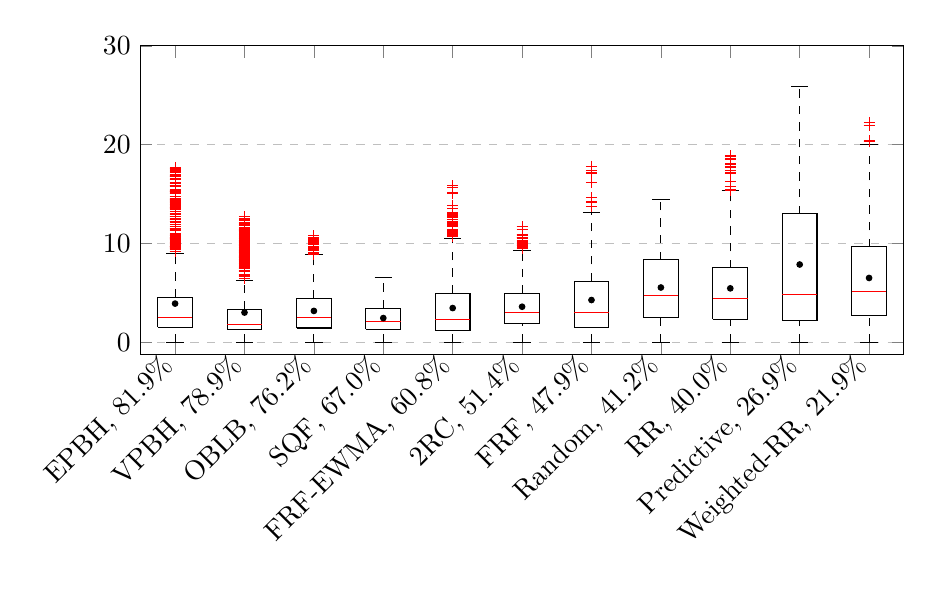
\begin{tikzpicture}[scale=1,transform shape]
\pgfplotsset{grid style={dashed}}
\begin{axis}[%
width=0.93\columnwidth,
height=5.5cm,
xmin=0.5, 
xmax=11.5,
ymin=-1.2, 
ymax=30,
xlabel style = {center},
xtick={1,2,3,4,5,6,7,8,9,10,11,12},
xticklabels={%
{EPBH, $81.9\%$},%
{VPBH, $78.9\%$},%
{OBLB, $76.2\%$},%
{SQF, $67.0\%$},%
{FRF-EWMA, $60.8\%$},%
{2RC, $51.4\%$},%
{FRF, $47.9\%$},%
{Random, $41.2\%$},%
{RR, $40.0\%$},%
{Predictive, $26.9\%$},%
{Weighted-RR, $21.9\%$}%
},
x tick label style={rotate=45, anchor=east},
ymajorgrids,
]
\addplot [
color=black,
dashed
]
coordinates{
 (1,4.57617)(1,9.02788) 
};

\addplot [
color=black,
dashed
]
coordinates{
 (2,3.34152)(2,6.26943) 
};

\addplot [
color=black,
dashed
]
coordinates{
 (3,4.43125)(3,8.86237) 
};

\addplot [
color=black,
dashed
]
coordinates{
 (4,3.465)(4,6.58852) 
};

\addplot [
color=black,
dashed
]
coordinates{
 (5,4.97803)(5,10.5269) 
};

\addplot [
color=black,
dashed
]
coordinates{
 (6,4.92883)(6,9.33183) 
};

\addplot [
color=black,
dashed
]
coordinates{
 (7,6.21138)(7,13.1455) 
};

\addplot [
color=black,
dashed
]
coordinates{
 (8,8.35872)(8,14.4421) 
};

\addplot [
color=black,
dashed
]
coordinates{
 (9,7.54385)(9,15.3635) 
};

\addplot [
color=black,
dashed
]
coordinates{
 (10,13.0111)(10,25.8548) 
};

\addplot [
color=black,
dashed
]
coordinates{
 (11,9.66816)(11,19.9898) 
};

\addplot [
color=black,
dashed
]
coordinates{
 (1,0)(1,1.53656) 
};

\addplot [
color=black,
dashed
]
coordinates{
 (2,0)(2,1.32854) 
};

\addplot [
color=black,
dashed
]
coordinates{
 (3,0)(3,1.4642) 
};

\addplot [
color=black,
dashed
]
coordinates{
 (4,0)(4,1.33472) 
};

\addplot [
color=black,
dashed
]
coordinates{
 (5,0)(5,1.23414) 
};

\addplot [
color=black,
dashed
]
coordinates{
 (6,0)(6,1.91124) 
};

\addplot [
color=black,
dashed
]
coordinates{
 (7,0)(7,1.54043) 
};

\addplot [
color=black,
dashed
]
coordinates{
 (8,0)(8,2.48405) 
};

\addplot [
color=black,
dashed
]
coordinates{
 (9,0)(9,2.32885) 
};

\addplot [
color=black,
dashed
]
coordinates{
 (10,0)(10,2.24439) 
};

\addplot [
color=black,
dashed
]
coordinates{
 (11,0)(11,2.69095) 
};

\addplot [
color=black,
solid
]
coordinates{
 (0.875,9.02788)(1.125,9.02788) 
};

\addplot [
color=black,
solid
]
coordinates{
 (1.875,6.26943)(2.125,6.26943) 
};

\addplot [
color=black,
solid
]
coordinates{
 (2.875,8.86237)(3.125,8.86237) 
};

\addplot [
color=black,
solid
]
coordinates{
 (3.875,6.58852)(4.125,6.58852) 
};

\addplot [
color=black,
solid
]
coordinates{
 (4.875,10.5269)(5.125,10.5269) 
};

\addplot [
color=black,
solid
]
coordinates{
 (5.875,9.33183)(6.125,9.33183) 
};

\addplot [
color=black,
solid
]
coordinates{
 (6.875,13.1455)(7.125,13.1455) 
};

\addplot [
color=black,
solid
]
coordinates{
 (7.875,14.4421)(8.125,14.4421) 
};

\addplot [
color=black,
solid
]
coordinates{
 (8.875,15.3635)(9.125,15.3635) 
};

\addplot [
color=black,
solid
]
coordinates{
 (9.875,25.8548)(10.125,25.8548) 
};

\addplot [
color=black,
solid
]
coordinates{
 (10.875,19.9898)(11.125,19.9898) 
};

\addplot [
color=black,
solid
]
coordinates{
 (0.875,0)(1.125,0) 
};

\addplot [
color=black,
solid
]
coordinates{
 (1.875,0)(2.125,0) 
};

\addplot [
color=black,
solid
]
coordinates{
 (2.875,0)(3.125,0) 
};

\addplot [
color=black,
solid
]
coordinates{
 (3.875,0)(4.125,0) 
};

\addplot [
color=black,
solid
]
coordinates{
 (4.875,0)(5.125,0) 
};

\addplot [
color=black,
solid
]
coordinates{
 (5.875,0)(6.125,0) 
};

\addplot [
color=black,
solid
]
coordinates{
 (6.875,0)(7.125,0) 
};

\addplot [
color=black,
solid
]
coordinates{
 (7.875,0)(8.125,0) 
};

\addplot [
color=black,
solid
]
coordinates{
 (8.875,0)(9.125,0) 
};

\addplot [
color=black,
solid
]
coordinates{
 (9.875,0)(10.125,0) 
};

\addplot [
color=black,
solid
]
coordinates{
 (10.875,0)(11.125,0) 
};

\addplot [
color=black,
solid
]
coordinates{
 (0.75,1.53656)(0.75,4.57617)(1.25,4.57617)(1.25,1.53656)(0.75,1.53656) 
};

\addplot [
color=black,
solid
]
coordinates{
 (1.75,1.32854)(1.75,3.34152)(2.25,3.34152)(2.25,1.32854)(1.75,1.32854) 
};

\addplot [
color=black,
solid
]
coordinates{
 (2.75,1.4642)(2.75,4.43125)(3.25,4.43125)(3.25,1.4642)(2.75,1.4642) 
};

\addplot [
color=black,
solid
]
coordinates{
 (3.75,1.33472)(3.75,3.465)(4.25,3.465)(4.25,1.33472)(3.75,1.33472) 
};

\addplot [
color=black,
solid
]
coordinates{
 (4.75,1.23414)(4.75,4.97803)(5.25,4.97803)(5.25,1.23414)(4.75,1.23414) 
};

\addplot [
color=black,
solid
]
coordinates{
 (5.75,1.91124)(5.75,4.92883)(6.25,4.92883)(6.25,1.91124)(5.75,1.91124) 
};

\addplot [
color=black,
solid
]
coordinates{
 (6.75,1.54043)(6.75,6.21138)(7.25,6.21138)(7.25,1.54043)(6.75,1.54043) 
};

\addplot [
color=black,
solid
]
coordinates{
 (7.75,2.48405)(7.75,8.35872)(8.25,8.35872)(8.25,2.48405)(7.75,2.48405) 
};

\addplot [
color=black,
solid
]
coordinates{
 (8.75,2.32885)(8.75,7.54385)(9.25,7.54385)(9.25,2.32885)(8.75,2.32885) 
};

\addplot [
color=black,
solid
]
coordinates{
 (9.75,2.24439)(9.75,13.0111)(10.25,13.0111)(10.25,2.24439)(9.75,2.24439) 
};

\addplot [
color=black,
solid
]
coordinates{
 (10.75,2.69095)(10.75,9.66816)(11.25,9.66816)(11.25,2.69095)(10.75,2.69095) 
};

\addplot [
color=red,
solid
]
coordinates{
 (0.75,2.5132)(1.25,2.5132) 
};

\addplot [
color=red,
solid
]
coordinates{
 (1.75,1.85185)(2.25,1.85185) 
};

\addplot [
color=red,
solid
]
coordinates{
 (2.75,2.53327)(3.25,2.53327) 
};

\addplot [
color=red,
solid
]
coordinates{
 (3.75,2.11353)(4.25,2.11353) 
};

\addplot [
color=red,
solid
]
coordinates{
 (4.75,2.33437)(5.25,2.33437) 
};

\addplot [
color=red,
solid
]
coordinates{
 (5.75,3.04626)(6.25,3.04626) 
};

\addplot [
color=red,
solid
]
coordinates{
 (6.75,3.07519)(7.25,3.07519) 
};

\addplot [
color=red,
solid
]
coordinates{
 (7.75,4.77691)(8.25,4.77691) 
};

\addplot [
color=red,
solid
]
coordinates{
 (8.75,4.41638)(9.25,4.41638) 
};

\addplot [
color=red,
solid
]
coordinates{
 (9.75,4.88217)(10.25,4.88217) 
};

\addplot [
color=red,
solid
]
coordinates{
 (10.75,5.13182)(11.25,5.13182) 
};

\addplot [
color=black,
only marks,
mark=+,
mark options={solid,draw=red}
]
coordinates{
 (1,9.18481)(1,9.22624)(1,9.38466)(1,9.47905)(1,9.48457)(1,9.58649)(1,9.61326)(1,9.66827)(1,9.72465)(1,9.72495)(1,9.72798)(1,9.74365)(1,9.77867)(1,9.90183)(1,10.0021)(1,10.0104)(1,10.1004)(1,10.1242)(1,10.1685)(1,10.3283)(1,10.3672)(1,10.4384)(1,10.4928)(1,10.4954)(1,10.5056)(1,10.5832)(1,10.5879)(1,10.6038)(1,10.765)(1,10.8621)(1,10.8996)(1,11.0463)(1,11.2948)(1,11.3794)(1,11.4893)(1,11.5059)(1,11.7601)(1,11.9367)(1,12.1842)(1,12.2455)(1,12.4377)(1,12.4802)(1,12.5383)(1,12.7196)(1,12.7801)(1,12.9042)(1,13.0555)(1,13.2203)(1,13.4767)(1,13.569)(1,13.5716)(1,13.6303)(1,13.6727)(1,13.6915)(1,13.7184)(1,13.81)(1,13.9546)(1,13.9884)(1,14.0545)(1,14.1604)(1,14.1626)(1,14.2105)(1,14.2718)(1,14.3264)(1,14.3416)(1,14.4191)(1,14.4381)(1,14.4636)(1,14.5252)(1,14.5958)(1,14.7372)(1,15.0872)(1,15.0928)(1,15.1194)(1,15.2394)(1,15.2786)(1,15.2795)(1,15.2827)(1,15.3195)(1,15.3493)(1,15.4991)(1,15.736)(1,15.8323)(1,15.8994)(1,16.0633)(1,16.2017)(1,16.4445)(1,16.4992)(1,16.626)(1,16.7615)(1,16.7781)(1,16.7994)(1,16.9281)(1,16.9292)(1,17.0079)(1,17.1615)(1,17.2805)(1,17.3798)(1,17.4417)(1,17.5597)(1,17.5752)(1,17.693) 
};

\addplot [
color=black,
only marks,
mark=+,
mark options={solid,draw=red}
]
coordinates{
 (2,6.4717)(2,6.66573)(2,6.69161)(2,6.69447)(2,6.71805)(2,6.809)(2,6.81715)(2,6.82031)(2,6.85045)(2,6.87271)(2,7.13985)(2,7.21434)(2,7.28104)(2,7.30433)(2,7.30815)(2,7.47427)(2,7.47793)(2,7.49159)(2,7.50966)(2,7.60983)(2,7.61358)(2,7.61719)(2,7.66044)(2,7.7149)(2,7.73391)(2,7.80038)(2,7.89834)(2,7.93831)(2,7.99071)(2,8.02781)(2,8.11195)(2,8.13368)(2,8.18727)(2,8.26116)(2,8.30566)(2,8.35307)(2,8.3619)(2,8.36918)(2,8.43342)(2,8.46526)(2,8.54682)(2,8.55436)(2,8.5714)(2,8.61342)(2,8.62478)(2,8.65001)(2,8.70991)(2,8.72873)(2,8.73844)(2,8.7541)(2,8.76339)(2,8.83812)(2,8.91936)(2,8.96649)(2,9.02105)(2,9.06236)(2,9.07488)(2,9.12067)(2,9.1302)(2,9.15755)(2,9.20855)(2,9.21018)(2,9.24776)(2,9.25204)(2,9.27738)(2,9.29335)(2,9.39018)(2,9.3943)(2,9.49663)(2,9.58407)(2,9.59252)(2,9.63348)(2,9.65515)(2,9.76568)(2,9.82976)(2,9.83776)(2,9.85016)(2,9.89164)(2,9.89338)(2,9.93122)(2,9.94496)(2,10.0004)(2,10.1097)(2,10.1431)(2,10.1531)(2,10.2051)(2,10.2248)(2,10.2441)(2,10.2711)(2,10.3189)(2,10.3247)(2,10.3379)(2,10.4598)(2,10.4746)(2,10.5437)(2,10.6402)(2,10.6772)(2,10.7592)(2,10.8046)(2,10.8822)(2,10.9307)(2,10.9791)(2,11.1757)(2,11.2296)(2,11.284)(2,11.3076)(2,11.345)(2,11.3628)(2,11.374)(2,11.4463)(2,11.4534)(2,11.4687)(2,11.5322)(2,11.5518)(2,11.5923)(2,11.846)(2,11.8562)(2,11.8579)(2,11.881)(2,11.9322)(2,11.9916)(2,12.0674)(2,12.1387)(2,12.3692)(2,12.3931)(2,12.5033)(2,12.7269) 
};

\addplot [
color=black,
only marks,
mark=+,
mark options={solid,draw=red}
]
coordinates{
 (3,8.92423)(3,9.03246)(3,9.07936)(3,9.27965)(3,9.35633)(3,9.37381)(3,9.46564)(3,9.54691)(3,9.66094)(3,9.91854)(3,9.92763)(3,9.93013)(3,9.93843)(3,9.97669)(3,9.98116)(3,10.1406)(3,10.1706)(3,10.2908)(3,10.3603)(3,10.4811)(3,10.5)(3,10.5218)(3,10.5705)(3,10.5994)(3,10.6257)(3,10.6442)(3,10.7788)(3,10.8096) 
};

\addplot [
color=black,
only marks,
mark=+,
mark options={solid,draw=red}
]
coordinates{
 (5,10.7222)(5,10.7483)(5,10.7728)(5,10.8736)(5,10.943)(5,11.0087)(5,11.1121)(5,11.2089)(5,11.2815)(5,11.3108)(5,11.355)(5,11.359)(5,11.4261)(5,11.7609)(5,11.7732)(5,11.826)(5,11.8505)(5,11.9477)(5,12.0618)(5,12.0679)(5,12.12)(5,12.1515)(5,12.2779)(5,12.4337)(5,12.6522)(5,12.6925)(5,12.7095)(5,12.7384)(5,12.7513)(5,12.8001)(5,12.9882)(5,13.0156)(5,13.1445)(5,13.5709)(5,13.8392)(5,15.1151)(5,15.6425)(5,15.8431) 
};

\addplot [
color=black,
only marks,
mark=+,
mark options={solid,draw=red}
]
coordinates{
 (6,9.50955)(6,9.61863)(6,9.75796)(6,9.75899)(6,9.87853)(6,9.95741)(6,10.0281)(6,10.07)(6,10.2443)(6,10.2778)(6,10.5438)(6,10.5869)(6,10.594)(6,10.6358)(6,10.8423)(6,10.9154)(6,10.9611)(6,11.4336)(6,11.6992) 
};

\addplot [
color=black,
only marks,
mark=+,
mark options={solid,draw=red}
]
coordinates{
 (7,13.7568)(7,14.1959)(7,14.2137)(7,14.6465)(7,16.169)(7,17.08)(7,17.1403)(7,17.3695)(7,17.8344) 
};

\addplot [
color=black,
only marks,
mark=+,
mark options={solid,draw=red}
]
coordinates{
 (9,15.4095)(9,15.4553)(9,15.4753)(9,15.7309)(9,16.2663)(9,17.0679)(9,17.1209)(9,17.1826)(9,17.4212)(9,17.7119)(9,17.8209)(9,18.014)(9,18.0994)(9,18.5358)(9,18.5389)(9,18.5472)(9,18.6006)(9,18.7701)(9,18.8817) 
};

\addplot [
color=black,
only marks,
mark=+,
mark options={solid,draw=red}
]
coordinates{
 (11,20.2959)(11,20.3354)(11,20.376)(11,21.9593)(11,22.2474) 
};

\addplot [
color=black,
only marks,
mark=*,
mark options={solid},
mark size = {1pt},
]
coordinates{
 (1,3.93244)(2,3.02403)(3,3.19245)(4,2.47096)(5,3.48272)(6,3.61642)(7,4.29458)(8,5.56012)(9,5.47445)(10,7.88444)(11,6.52479) 
};

\end{axis}
\end{tikzpicture}

  \vspace{-4mm}
\caption{Box plots of the maximum response time in all the replicas
  for every control interval. Each box depicts from the first quartile
  to the third. The red line shows the median; outliers are
  represented with red crosses while the black dots indicate the
  average value (also considering the outliers).}
  \vspace{-2mm}
\label{fig:clientchanges-boxplot}
\end{figure}

The right column in Figure~\ref{fig:clientchanges-full} shows the
control variable $\theta_i$ for each replica, while the left column
shows the effective weights $w_i$ that have been assigned by the
load-balancing strategies. Since solutions like the Round Robin do not
assign directly the weights, we decided to compute the effective
values that can be found after the load-balancing assignments. 

The algorithms are ordered based on the percentage $\%_{oc}$ of optional
content served, where the Equality Principle-Based Heuristic (EPBH)
achieves the best percentage overall, followed by the Variational
Principle-Based Heuristic (VPBH) and by the Optimization Based
Load-Balancer (OBLB).

For this scenario, the strategies that are aware of the adaptation at
the replica level achieve better results in terms of percentage of
optional content served. The Shortest Queue First (SQF) algorithm is
the only existing one capable of achieving similar (yet lower)
performance in terms of optional content delivered.

To analyze the effect of the load-balancing strategies on the replicas
response times, Figure~\ref{fig:clientchanges-boxplot} shows a box
plot of the maximum response time experienced in intervals of time by the
replicas. The load-balancing strategies are ordered from left to right
based on the percentage of optional code $\%_{oc}$ achieved. As in
every box plot, the bottom line for each box represents the first
quartile, the top line the third and the red line is the median. The
red crosses depict the outliers. In addition to the classical box plot
information, the black dots depict for each algorithm the average
value of the maximum response time measured during the experiment, also
considering the outliers.

The box plots clearly show that all the solutions presented in this
paper achieve distributions that have outliers, as well as almost all
the literature ones. The only exception seems to be SQF, that achieves
predictable maximum response time, with a median that is just slightly
higher than the one achieved by VPBH. OBLB offers in this case a
compromise between optional content and the presence of outliers, that
are limited with respect to all the other solutions. EPBH offers the
highest percentage of optional content served, by sacrificing the
response time bound. From this additional information one can conclude that
the solutions presented in this paper should be used carefully in
situations where the requirement on the response time is not soft, but
increase the profit of the application developer (up to $15\%$ more
optional code served with respect to the best state of the art
solution for the case study). Notice also that the proposed heuristics
(EPBH and VPBH) have tunable parameters that can be used to exploit
the trade-off between response time bounds and optional content served.

Notice that this case study features only a limited number of
replicas. However, we have conducted additional tests, also in more
complex scenarios, reporting results similar to the ones presented
herein. In the next section we test the effect of infrastructural
changes to load-balancing solutions and response times.

\subsection{Reacting to infrastructure resources}

In the second case study the architecture is composed of five
replicas. At time $0$s, $\phi_1 = 0.07$s, $\psi_1 = 0.001$s. The
second and third replicas are slower and have $\phi_{2,3} = 0.14$s and
$\psi_{2,3} = 0.002$s. The fourth and fifth replicas are the slowest
with $\phi_{4,5} = 0.7$s and $\psi_{4,5} = 0.01$s.

At time $250$s the amount of resources assigned to the first replica
is decreased, therefore $\phi_1 = 0.35$s and $\psi_1 = 0.005$s. At
time $500$s, the fifth replica receives more resources, achieving
$\phi_5 = 0.07$s and $\psi_5 = 0.001$s. The same happens at time $750$
to the fourth replica.

\begin{table}
\centering
\caption{Performance with variable infrastructure resources}
\label{tab:resourcechanges-performance}
\begin{tabular}{l c c c}
\hline
Algorithm   & $\%_{oc}$ & $\mu_u$ & $\sigma_u$ \\
\hline
OBLB        & $\mathbf{91.4\%}$ & $0.71$          & $0.89$ \\
EPBH        & $89.5\%$          & $1.06$          & $1.95$ \\
VPBH        & $87.7\%$          & $1.02$          & $1.90$ \\
SQF         & $83.3\%$          & $\mathbf{0.55}$ & $\mathbf{0.40}$ \\
RR          & $75,5\%$          & $1.11$          & $2.42$ \\
Random      & $72.9\%$          & $0.86$          & $2.23$ \\
2RC         & $72.2\%$          & $0.74$          & $1.64$ \\
FRF         & $70.4\%$          & $1.27$          & $2.03$ \\
Weighted-RR & $60.7\%$          & $0.90$          & $2.97$ \\
FRF-EWMA    & $51.4\%$          & $1.44$          & $3.41$ \\
Predictive  & $47.4\%$          & $1.66$          & $3.48$ \\
\hline
\end{tabular}
\vspace{-4mm}
\end{table}

Table~\ref{tab:resourcechanges-performance} reports the percentage
$\%_{oc}$, the average response time and the user-perceived stability
for the different algorithms. It should be noted again that the
developed strategies obtain better optional content served, however
slightly penalizing response times. However, the Optimization Based
Load-Balancer is capable of obtaining both low response times and high
percentage of optional content served. This is due to the amount of
information that it uses, since we assume that the computation times
for mandatory and optional part are known. The optimization-based
strategy is capable of reacting fast to changes and achieves
predictability in the application behavior. Again, if one does not
have all the necessary information available, it is possible to
implement strategies that would better exploit the trade-off between
bounded response time and optional content.


\section{Conclusion}
\label{sec:conclusion}

\section*{Acknowledgement}
  This work was partially supported by the Swedish Research Council
  (VR) under contract number C0590801 for the project Cloud Control
  and through the LCCC Linnaeus Center. Also, we received partial
  support from the ELLIIT Excellence Center.

\printbibliography

\end{document}
